\documentclass[professionalfonts,compress,unicode]{beamer}

\usepackage{amsmath,amssymb}
\usepackage[utf8]{inputenc}
\usepackage[russian]{babel}
\usepackage{epstopdf}

\usetheme{Warsaw}
\usecolortheme{uranix}

\setbeamertemplate{headline}
{%
  \begin{beamercolorbox}[sep=0.3cm,wd=\paperwidth]{section in head/foot}%
    \usebeamerfont{frametitle}%
    \vbox{}\vskip-1ex%
    \strut\insertsectionhead\strut\par%
    \vskip-1ex%
  \end{beamercolorbox}%
}
\setbeamertemplate{navigation symbols}{}
\setbeamertemplate{footline}{}

\renewcommand{\thefootnote}{\fnsymbol{footnote}}

\graphicspath{{images//}}

\title[Погрешности. Дифференцирование]{Погрешности вычислений\\Численное дифференцирование}
\author[Цыбулин И.В.]{Скалько Юрий Иванович\\
\textbf{Цыбулин Иван}
}
\date{}
%\vspace{0.3cm}

\begin{document}

{
\setbeamertemplate{headline}[default]
\frame{
\titlepage
}

%\frame{
%\frametitle{Содержание}
%\small
%%\tiny
%\tableofcontents
%}
}

\newcommand\myframe[2]{\subsection{#1}\frame{\frametitle{#1}{#2}}}

\section{ }

\myframe{Материалы по курсу вычислительной математики}
{
\begin{itemize}
	\item 
		Материалы курса (методички, лекции, учебники и др.) можно найти 
		на сайте кафедры вычислительной математики
		{\color{blue} http://crec.mipt.ru/study/materials/compmath/}
	\item 
		Любые вопросы по курсу (и не только) можно присылать на почтовый ящик
		{\color{blue} tsybulin@crec.mipt.ru}
\end{itemize}
}

\section{Погрешности}
\myframe{Абсолютная и относительная погрешность}
{
Если про величину $X$ известно, что $X \in [\bar{X}-\frac{\Delta X}{2}, \bar{X}+\frac{\Delta X}{2}]$, то
\begin{itemize}
	\item \emph{абсолютной погрешностью} $X$ называется величина $\Delta X$
	\item \emph{относительной погрешностью} --- отношение $\frac{\Delta X}{\left|\bar{X}\right|}$
\end{itemize}
}

\myframe{Приближенные вычисления}
{
\begin{block}{Задача}
	Как вычислить сложную функцию (например, $f(x) = \sin x$) в некоторой заданной точке?
\end{block}

\begin{itemize}
	\pause \item Воспользоваться большой таблицей заранее посчитанных значений функций
	\pause 
	
	\alert{Но ведь эту таблицу необходимо еще составить!}
	\alert{Не ясно, как искать значения, которые в таблице отсутствуют}
	\pause \item Численно решить дифференциальное уравнение $y''(x) + y(x) = 0$
	\pause
	
	\alert{Пока совершенно не ясно, как это сделать (но это только пока!)}
	\pause \item Воспользоваться представлением в виде рядов 
	
	{\color[HTML]{008000} Простейший вариант --- воспользоваться рядом Тейлора}
	
\end{itemize}
}

\myframe{Ряд Тейлора}
{
	Для функции $\sin x$ ряд Тейлора в окрестности точки $x=0$ выглядит следующим образом
	$$
	\sin x = x - \frac{x^3}{6} + \frac{x^5}{120} + \dots = \sum_{k=0}^{\infty} (-1)^k\frac{x^{2k+1}}{(2k+1)!}
	$$
	\pause
	\begin{block}{Вопрос}
	Какой радиус сходимости этого ряда?
	\pause
	
	$R = \infty$, Ряд сходится при любом $x$
	\end{block}
	\begin{itemize}
	\pause\item Но как суммировать бесконечный ряд на практике?
	\pause\item Ограничимся только несколькими членами этого ряда
	\pause\item Необходимо оценить ошибку, допущенную при этом
	\end{itemize}
}

\myframe{Практический метод}
{
	Итак, для приближенного вычисления $\sin x$ можно просуммировать 
	несколько первых членов ряда Тейлора. Для оценки ошибки воспользуемся 
	формулой Тейлора с остаточным членом в форме Лагранжа
	
	$$
	\sin x = \underbrace{\sum_{k=0}^{n} (-1)^k \frac{x^{2k+1}}{(2k+1)!}}_{S_n} + 
	\frac{x^{2n+2}}{(2n+2)!}\sin^{(2n+2)} \xi, 
	\quad \xi \in [0, x]
	$$
	
	\pause
	
	Отбросив остаточный член, мы тем самым допускаем ошибку 
	$$
	\left|\frac{x^{2n+2}}{(2n+2)!}\sin^{(2n+2)} \xi \right| \leq 
	\frac{x^{2n+2}}{(2n+2)!}M_{2n+2} \equiv \varepsilon_{\text{метод}} 
	$$
	Здесь для максимума модуля $2n+2$-й производной использовано стандартное в 
	вычислительной математике обозначение $M_{2n+2}$.
}

\myframe{Погрешность метода}
{
	Ошибка $\varepsilon_{\text{метод}}$ обусловлена тем, что метод, который мы 
	применяем для вычисления значения функции является \emph{неточным}.
	Данная ошибка является \emph{ошибкой метода} (или \emph{погрешностью метода})
	
	\pause
	
	Так как все производные функции $\sin x$ ограничены по модулю единицей, $M_{2n+2} = 1$ и 
	$$
	\varepsilon_{\text{метод}} = \frac{x^{2n+2}}{(2n+2)!}
	$$
	При стремлении $n \rightarrow \infty$ ошибка метода начиная с $n = n_0 >
	x/2$ монотонно стремится к нулю.
}

\myframe{Проверка}
{
	Для проверки посчитаем $\sin \frac{\pi}{2}$ суммируя до $50$ членов ряда. 
	
	\begin{figure}%
	\center
	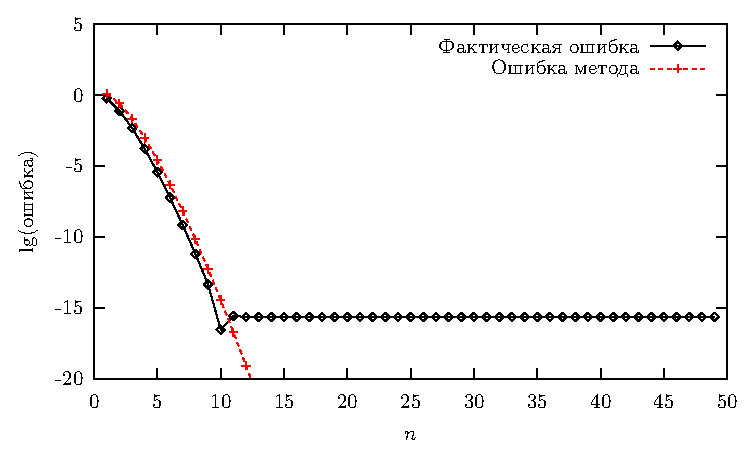
\includegraphics[height=0.5\textheight]{sine_pi_2}
	\end{figure}
	
	После сложения $10$ членов ряда фактическая ошибка составила $10^{-16}$ и перестала уменьшаться. 
	Такое поведение говорит про наличие еще какой-то погрешности, кроме ошибки метода. 
	\begin{block}{}
	Но ведь $10^{-16}$ это же совсем немного? Или нет?
	\end{block}
}

\myframe{Проверка №2}
{
	Проделаем аналогичные вычисления, но уже для $\sin \frac{17\pi}{2}$
	\footnote{$x = \frac{17\pi}{2} \approx 26.7$}
	
	\begin{figure}%
	\center
	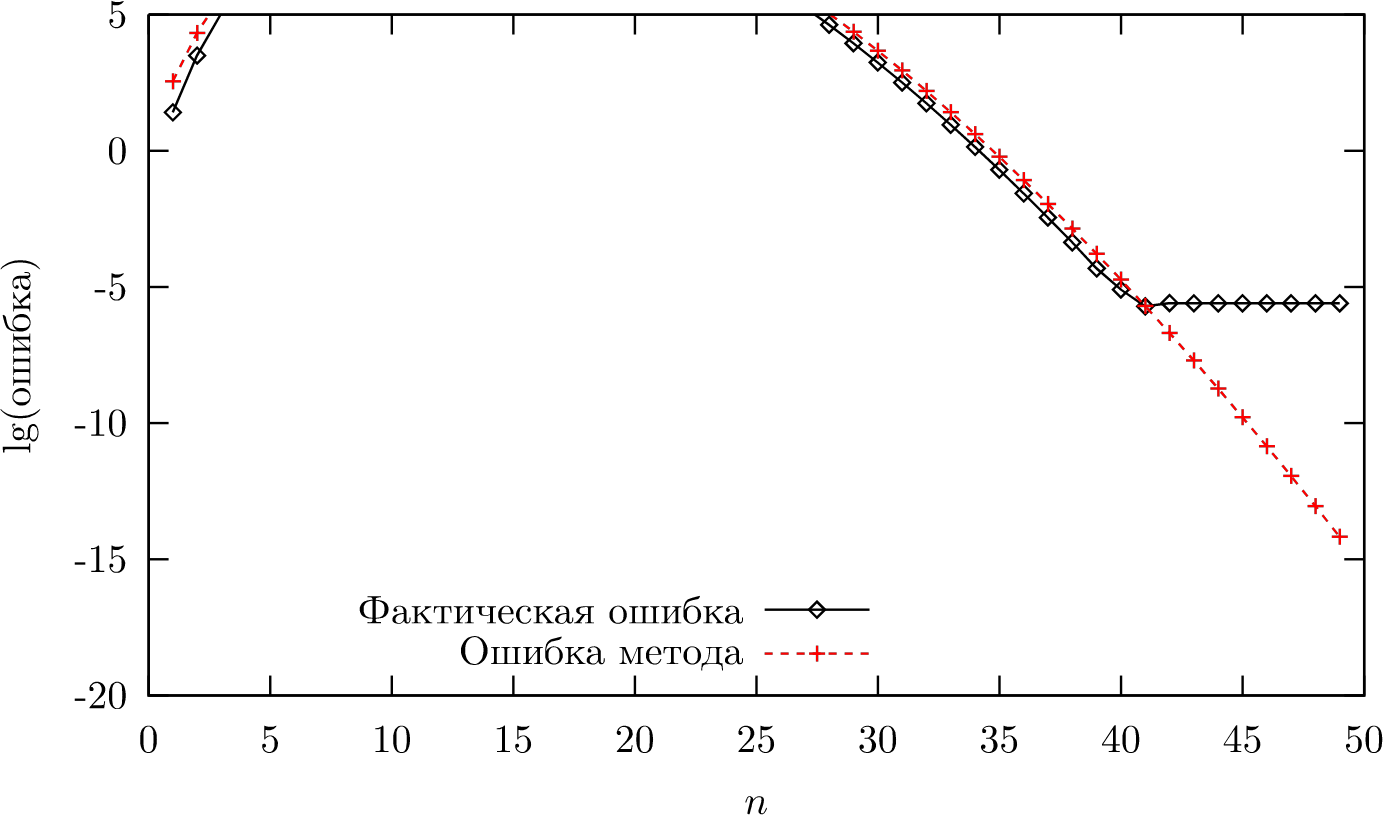
\includegraphics[height=0.5\textheight]{sine_17pi_2}
	\end{figure}
	
	Теперь ошибка перестает уменьшаться после 40 слагаемого и составляет уже $10^{-6}$.
	Определенно, данная ошибка может стать серьезной проблемой.
}

\myframe{Машинная арифметика}
{
	До сих пор все вычисления мы рассматривали в \emph{идеальной арифметике}, где все математические 
	операции производятся \emph{абсолютно точно}. На практике, приходится иметь дело с машинной арифметикой,
	которая оперирует с \emph{приближенными} значениями чисел. Чаще всего, числа представлены в 
	вычислительной технике в виде \emph{чисел с плавающей запятой} (floating-point values). Каждое число хранится 
	в виде
	$$
	x = s \cdot 2^e,
	$$
	где $1 \leq s < 2$ - мантисса, число с фиксированным количеством знаков после запятой, $e$ - экспонента или показатель степени, 
	целое число. Поскольку целая часть мантиссы всегда равна 1, число значащих цифр в машинном представлении $x$ всегда совпадает с
	количеством знаков в мантиссе.
}

\myframe{Машинная арифметика в вычислениях}
{
	На практике, хранение чисел в форме с плавающей запятой приводит к хранению каждого числа с фиксированной относительной погрешностью.
	Например, в десятичной системе, если в мантиссе числа 5 значащих цифр (не считая первой единицы), 
	то относительная погрешность хранения данного числа составляет $10^{-5}$
	$$
	1.23456 \cdot 10^{78} = (1.23456 \pm 0.000005) \cdot 10^{78}
	$$
	$$
	\bar X = 1.23456 \cdot 10^{78}, \, 
	\Delta X = 0.00001 \cdot 10^{78}, \,
	$$
	$$
	\frac{\Delta X}{|\bar X|} = \frac{0.00001\cdot 10^{78}}{1.23456\cdot 10^{78}} = \frac{0.00001}{1.23456} < 10^{-5}
	$$
}

\myframe{Машинная арифметика в вычислениях}
{
	Аналогично, только с использованием двоичной, а не десятичной системы счисления, определяются
	относительные погрешности хранения стандартных числе с плавающей запятой
	\begin{itemize}
		\item тип single или float (32 бита) - мантисса имеет 23 значащих бита, 
		относительная погрешность составляет $2^{-23} \approx 1.2 \cdot 10^{-7}$
		\item тип double (64 бита) - мантисса имеет 53 значащих бита, 
		относительная погрешность составляет $2^{-53} \approx 1.1 \cdot 10^{-16}$
	\end{itemize}
	
	\pause
	Теперь понятно, что ошибка $10^{-16}$, которую мы получили при вычислении $\sin \frac{\pi}{2}$ есть 
	просто погрешность вычислений, обусловленная неточным представлением чисел в вычислительной технике.
	
	\pause
	Но как объяснить ошибку $10^{-6}$, которую мы получили, вычисляя $\sin \frac{17\pi}{2}$?
}

\myframe{Ошибка округления}
{
	Так как округление до 16 значащих цифр\footnote{подразумеваем операции с double} происходит при \emph{каждой} операции, 
	необходимо подсчитать суммарную ошибку округления всех слагаемых. Поскольку заранее неизвестно, в какую сторону происходит округление,
	необходимо сложить погрешности округления по модулю.
	\pause
	
	Ошибка округления числа $X$ не превосходит $2^{-K}|X|$, где $K$ - число значащих бит в мантиссе (в нашем случае 53). Оценим ошибку округления 
	$S_n$.
	
	$$
	S_n = \sum_{k=0}^{n} (-1)^k\frac{x^{2k+1}}{(2k+1)!}
	$$
	$$
	\varepsilon_{\text{округ}} = \sum_{k=0}^{n} \left| 2^{-K}(-1)^k\frac{x^{2k+1}}{(2k+1)!} \right| = 
	2^{-K}\sum_{k=0}^{n} \frac{x^{2k+1}}{(2k+1)!} \approx 2^{-K} \sh x 
	$$
}

\myframe{Ошибка округления}
{
	Итак, хотя исходный ряд был знакопеременным, и по модулю сумма ряда не превосходила единицы, 
	отдельные слагаемые могли достигать весьма существенных	значений по модулю.
	
	$$
	\max_{k} \frac{x^{2k+1}}{(2k+1)!} \approx \frac{x^x}{x!} \approx \frac{x^x}{\sqrt{2\pi x}\left(\frac{x}{e}\right)^x} = \frac{e^x}{\sqrt{2\pi x}}
	$$
	\pause
	Возвращаясь к случаю $\sin \frac{17\pi}{2}$, $x \approx 26.7$
	$$
	\frac{e^x}{\sqrt{2\pi x}} = 3 \cdot 10^{10}.
	$$
	Погрешность округления только этого слагаемого $\varepsilon_{\text{округ}} = 2^{-53} \times 3 \cdot 10^{10} \approx 3.3 \cdot 10^{-6}$, 
	что вполне соответствует фактической ошибке при вычислении $\sin \frac{17\pi}{2}$. 
}

\myframe{Вывод}
{
	Практически все прикладные задачи , которые приходится решать в рамках вычислительной математики, невозможно решить точно. 
	Этому препятствует два основных источника погрешности --- неточные(приближенные) методы и неидеальная(машинная) арифметика.
	Ошибке метода соответствует погрешность решения задачи в идеальной арифметике (в которой все действия выполняются точно).
	В ошибку округления входят погрешности всех вычислений при реализации данного метода.
}

\section{Численное дифференцирование}
\myframe{Производная}
{
	\begin{block}{Задача}
	Допустим, задана функция $f(x)$, то есть мы можем вычислить ее значение в любой точке $x$. 
	Как вычислить ее производную в заданной точке $x_0$?
	\end{block}
	\pause
	Вспомним определение производной
	$$
	f'(x_0) = \lim_{\delta \rightarrow 0} \frac{f(x_0+\delta) - f(x_0)}{\delta}
	$$
	\begin{block}{Вопрос}
	Какие еще определения производной Вы знаете?
	\end{block}
}

\myframe{Численный метод}
{
	$$
	f'(x_0) = \lim_{\delta \rightarrow 0} \frac{f(x_0+\delta) - f(x_0)}{\delta}
	$$
	Поиск предела, так же как и суммирование бесконечной суммы, является нетривиальной операцией.
	
	\pause
	Заменим предел значением отношения при некотором маленьком значении $\delta = h > 0$.
	
	$$
	f'(x_0) \approx \frac{f(x_0+h) - f(x)}{h}
	$$
}

\myframe{Ошибка метода}
{
	В первую очередь, нас интересует ошибка метода, которая возникает в результате замены предела 
	фиксированной разностью. Здесь нам снова поможет формула Тейлора. Разложим $f(x)$ в окрестности
	точки $x = x_0$.
	
	$$
	f(x) = f(x_0) + (x-x_0) f'(x_0) + \frac{(x-x_0)^2}{2} f''(\xi), \quad \xi \in [x_0,x]
	$$
	\pause
	Подставляя $x = x_0 + h$

	$$
	f(x_0 + h) = f(x_0) + h f'(x_0) + \frac{h^2}{2} f''(\xi), \quad \xi \in [x_0,x_0+h]
	$$
}

\myframe{Ошибка метода}
{
	$$
	f(x_0 + h) = f(x_0) + h f'(x_0) + \frac{h^2}{2} f''(\xi), \quad \xi \in [x_0,x_0+h]
	$$
	
	Группируем и делим на $h$
	
	$$
	\frac{f(x_0 + h) - f(x_0)}{h} - f'(x_0) = \frac{h}{2} f''(\xi)
	$$

	$$
	\varepsilon_{\text{метод}} = \left|\frac{f(x_0 + h) - f(x_0)}{h} - f'(x_0) \right| = \left |\frac{h}{2} f''(\xi) \right | \leq \frac{M_2 h}{2}
	$$
	
	Чем меньше $h$, тем меньшим оказывается погрешность метода. Погрешность метода линейно зависит от $h$. 
}

\myframe{Метод неопределенных коэффициентов}
{
	Будем искать другие способы вычисления производной. Допустим, мы хотим построить наиболее 
	точный метод для вычисления производной, который бы использовал значения функции в трех точках --- 
	в $x_0, x_0+h$ и $x_0-h$.
	
	Некоторые соображения о том, в каком виде следует искать требуемый метод дают свойства оператора дифференцирования.
	Известно, что операция дифференцирования линейна, т.е.
	$$
	(\alpha f + \beta g)' = \alpha f' + \beta g'
	$$
	Вполне логично искать \emph{линейную} формулу дифференцирования, т.е. такую, в которую значения дифференцируемой функции входят 
	\emph{линейно}
}

\myframe{Метод неопределенных коэффициентов}
{
	Запишем линейную функцию от $f(x_0), f(x_0+h), f(x_0-h)$ в виде линейной комбинации с неопределенными коэффициентами
	$$
	f'(x_0) \approx \alpha f(x_0-h)  + \beta f(x_0) + \gamma f(x_0+h)
	$$
	За счет надлежащего выбора $\alpha, \beta, \gamma$ добьемся максимального совпадения левой и правой части равенства.
	
	\pause
	Потребуем совпадения максимального количества членов в представлении в виде формулы Тейлора в точке $x_0$ левой и правой частей.
	\begin{block}{Замечание}
	Здесь делается предположение, что у функции $f(x)$ существует достаточное количество производных в точке $x_0$. 
	Необходимо иметь в виду, что если функция $f(x)$ не имеет всех необходимых производных, погрешность метода может увеличиваться.
	\end{block}
}

\myframe{\large Метод неопределенных коэффициентов. Формула Тейлора}
{
	$$
	f'(x_0) \approx \alpha f(x_0-h)  + \beta f(x_0) + \gamma f(x_0+h)
	$$
	Представляя значения в крайних точках с помощью формулы Тейлора
	$$
	f(x_0 \pm h) = f(x_0) \pm h f'(x_0) + \frac{h^2}{2} f''(x_0) \pm \frac{h^3}{6} f'''(\xi_{1,2})
	$$
	$$
	\xi_1 \in [x_0-h, x_0],\xi_2 \in [x_0, x_0+h]
	$$
	$$
	f'(x_0) \approx (\alpha + \beta + \gamma) f(x_0) + (\gamma - \alpha) h f'(x_0) + (\alpha+\gamma) \frac{h^2}{2}f''(x_0) + R
	$$
	$$
	R = \frac{h^3}{6}(\gamma f'''(\xi_2) - \alpha f'''(\xi_1))
	$$
}

\myframe{\large Метод неопределенных коэффициентов. Формула Тейлора}
{
	После исключения значений функции в крайних точках, приближенное равенство приобретает вид
	$$
	f'(x_0) \approx (\alpha + \beta + \gamma) f(x_0) + (\gamma - \alpha) h f'(x_0) + (\alpha+\gamma) \frac{h^2}{2}f''(x_0) + R
	$$
	$$
	R = \frac{h^3}{6}(\gamma f'''(\xi_2) - \alpha f'''(\xi_1))
	$$
	Потребуем, чтобы $\alpha + \beta + \gamma = 0, (\gamma - \alpha) h = 1, (\alpha+\gamma) \frac{h^2}{2} = 0$. 
	Искомые значения $\gamma = -\alpha = \frac{1}{2h}, \beta = 0$.
	При этом равенство превратится в 
	$$
	f'(x_0) \approx f'(x_0) + R
	$$
	Добавка $R$ как раз будет ошибкой метода. 
	$$
	\varepsilon_{\text{метод}} = |R| = \frac{h^3}{6} \frac{1}{2h}|f'''(\xi_2) + f'''(\xi_1)| \leq \frac{h^2}{6} M_3
	$$
}

\myframe{Формулы дифференцирования 1-го и 2-го порядков}
{
	Формула $f'(x_0) \approx \frac{f(x_0+h) - f(x_0)}{h}$ называется формулой односторонней разности, а
	$f'(x_0) \approx \frac{f(x_0 + h) - f(x_0 - h)}{2h}$ --- формулой центральной разности. Важное различие этих формул заключается
	в разной зависимости ошибки метода от $h$. Для односторонней разности эта зависимость линейная 
	$\varepsilon_{\text{метод}} \leq \frac{M_2 h}{2}$, в то время как для центральной --- квадратичная
	$\varepsilon_{\text{метод}} \leq \frac{M_3 h^2}{6}$.
	\pause
	
	Говорят, что формула односторонней разности имеет \emph{первый порядок аппроксимации},
	а центральной - \emph{второй порядок аппроксимации}
}

\myframe{Проверка}
{
	Проверим, действительно ли зависимость ошибки имеет такой характер для каждой из формул. Рассчитаем $\sin'1 = \cos 1$
	
	\begin{figure}%
	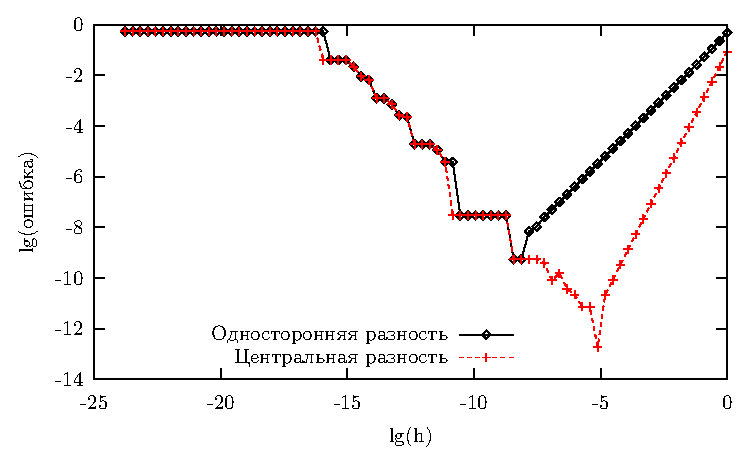
\includegraphics[height=0.5\textheight]{diff}%
	\end{figure}
	
	Оказывается, поведение ошибки имеет такой характер только при сравнительно больших $h$. Для односторонней разности при $h > 10^{-8}$,
	а для центральной --- при $h > 10^{-5}$. 
}

\myframe{Погрешности округления}
{
	Проще всего объяснить постоянное значение ошибки при использовании $h < 10^{-16}$. При данном значении величины 
	$x_0+h = 1+h$ и $x_0-h = 1-h$ округляются до $1$, при этом в числителе обеих формул стоит тождественный ноль 
	(вычитаются строго совпадающие значения), хотя реальное значение производной ненулевое.
	\pause
		
	Рассмотрим, какие ошибки округления возникают при вычислении по формуле односторонней разности. 
	$$
	f'(x_0) \approx \frac{f(x_0+h)-f(x_0)}{h}
	$$
	$$
	\varepsilon_{\text{округ}} = \frac{2^{-K}|f(x_0)|+2^{-K}|f(x_0+h)|}{h} \approx 2^{-K} \frac{2|f(x_0)|}{h}
	$$
	Аналогично для центральной разности
	$$
	\varepsilon_{\text{округ}} = \frac{2^{-K}|f(x_0-h)|+2^{-K}|f(x_0+h)|}{2h} \approx 2^{-K} \frac{|f(x_0)|}{h}
	$$
}

\myframe{Оптимальное значение h}
{
	Итак, при слишком маленьких значениях $h$ основной вклад в ошибку дает именно погрешность округления, которая
	растет с уменьшением $h$, а при слишком больших становится значительной ошибка метода. Найдем оптимальное значение
	$h$, при котором обе ошибки имеют одинаковую величину.
	\pause
	
	Для односторонней разности
	$$
	2^{-K} \frac{2|f(x_0)|}{h} = \varepsilon_{\text{округ}} = \varepsilon_{\text{метод}} = \frac{M_2 h}{2}
	$$
	$$
	h = \sqrt{2^{-K}\frac{4|f(x_0)|}{M_2}},\quad \varepsilon_{\text{сумм}} = 2 \sqrt{2^{-K} M_2 |f(x_0)|}
	$$
	Для проверки подставим $M_2 = |f(x_0)| = 1, K=53$, тогда
	$$h=2 \cdot 10^{-8},  \quad \varepsilon_{\text{сумм}} = 2 \cdot 10^{-8}$$
}

\myframe{Оптимальное значение h для формулы 2-го порядка}
{
	Для центральной разности
	$$
	2^{-K} \frac{|f(x_0)|}{h} = \varepsilon_{\text{округ}} = \varepsilon_{\text{метод}} = \frac{M_3 h^2}{6}
	$$
	$$
	h = \sqrt[3]{2^{-K}\frac{6|f(x_0)|}{M_3}},\quad \varepsilon_{\text{сумм}} = 2 \sqrt[3]{2^{-2K} \frac{M_3 |f(x_0)|^2}{6}}
	$$
	Для проверки подставим $M_2 = |f(x_0)| = 1, K=53$, тогда
	$$h=9 \cdot 10^{-6},  \quad \varepsilon_{\text{сумм}} = 2.5 \cdot 10^{-11}$$
}

\myframe{Вывод}
{
	Важно отметить, что при использовании формулы второго порядка удалось получить меньшую суммарную погрешность
	не выходя за пределы той же машинной точности что и в формуле первого порядка, то есть только за счет выбора 
	более качественного метода. 
	\pause
	
	Однако, не стоит забывать что функция, которую мы дифференцировали была достаточное 
	число раз (а именно 3 раза) непрерывно дифференцируема. Если формулу второго порядка применять
	к функции, у которой, например, $M_3 = \infty$, но $M_2 < \infty$, то оценка ошибки метода имела бы 
	такой же вид, как у формулы односторонней разности 1го порядка. В этом случае выигрыш был бы совсем 
	незначительным.
}

%%%%%%%%%%%%%%%%%%%%%%%%%%%%%%%%%%%%%%%%%%%%%%%
%%%%%%%%%%%%%%%%%%%%%%%%%%%%%%%%%%%%%%%%%%%%%%%
%%%%%%%%%                            %%%%%%%%%%
%%%%%%%%%%%%%%%%%%%%%%%%%%%%%%%%%%%%%%%%%%%%%%%
%%%%%%%%%%%%%%%%%%%%%%%%%%%%%%%%%%%%%%%%%%%%%%%
{
\setbeamertemplate{headline}[default] 
\frame{
	\begin{center}
	{\Huge Спасибо за внимание!}
	\end{center}
	\bigskip
	\begin{center}
	{\color{blue}{tsybulin@crec.mipt.ru}}
	\end{center}
	}
}

\end{document}
